\documentclass{article}
\usepackage[utf8]{inputenc}
\usepackage[T1]{fontenc}
\usepackage[czech]{babel}
\usepackage[utf8]{inputenc}
\usepackage{graphicx}
\usepackage{picture}
\usepackage{hyperref}
\usepackage{tabularx,ragged2e,booktabs,caption}
\usepackage{float}
\usepackage[table,xcdraw]{xcolor}
\bibliographystyle{czplain}
\usepackage[final]{pdfpages}
%\usepackage[left=3.5cm, text={14.5cm, 18cm},top=3cm]{geometry}
\usepackage[left=3cm,text={15.5cm,21cm},top=3cm]{geometry}
\renewcommand{\baselinestretch}{1.5}

\usepackage{titlesec}

\setcounter{secnumdepth}{4}

\titleformat{\paragraph}
{\normalfont\normalsize\bfseries}{\theparagraph}{1em}{}
\titlespacing*{\paragraph}
{0pt}{3.25ex plus 1ex minus .2ex}{1.5ex plus .2ex}

\usepackage{titlesec}
\newcommand{\sectionbreak}{\clearpage}

\begin{document}

%Titulna strana 
\begin{titlepage}

\begin{center}

\begin{figure}[h!]
\centering

\includegraphics[scale=0.15]{FIT.png}
\end{figure}
\vspace{\stretch{0.3}}

\Huge{\textbf {DHCP útoky\\}}
\vspace{\stretch{0.03}}
\huge{Přenos dat, počítačové sítě a protokoly\\}
\vspace{\stretch{0.03}}
\vspace{-1 mm}

\vspace{\stretch{0.618}}
\end{center}
\Large{
Bc. Bezák Adam\\
\hfill 2018}

\vspace{\stretch{0.065}}
\end{titlepage}

%\maketitle

\tableofcontents
\newpage

\section{Teoretická časť}

\subsection{DHCP - Dynamic Host Configuration Protocol}
Protokol DHCP sa používa na rýchľu, automatickú a centrálnu distribúciu IP adries skrz počítačovú sieť.Taktiež sa používa na nakonfigurovanie správnej masky siete, defaultnej brány a DNS servera.
DHCP komunikáciu je možné vidieť na obrázku \ref{fig:dhcp_session}.

\begin{figure}[h]
    \centering
    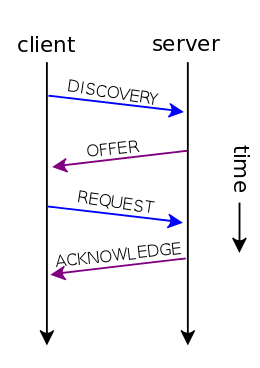
\includegraphics[width=100px]{pic/DHCP_session.png}
    \caption{DHCP komunikácia. }
    \label{fig:dhcp_session}
\end{figure}

Klient komunikuje skrz port 68 a server čaká na porte 67. Po pripojení zariadenia do siete, na ktorú je pripojený DHCP server, sa odošle packet s broadcast adresou zvaný \texttt{DHCPDISCOVER}. V momente keď tento packet dorazí na rozhranie DHCP serveru sa odošle z výstupného rozhrania packet s názvom \texttt{DHCPOFFER}, ktorý nesie informácie o možnej IP adrese, ktorá môže byť pridelená zariadeniu. Ak zariadenie tento packet príjme odpovie packetom \texttt{DHCPREQUEST}, ktorým žiada o pridelenie danej adresy. Ak mu server vyhovie odpovedá packetom \texttt{DHCPACK}. V opačnom prípade server odosiela packet \texttt{DHCPNACK} \cite{dhcp}.

\subsection{DHCP útoky}
Z uvedenej komunikácie je možné postrehnúť, že sa jedná o viacstavovú komunikáciu a tým pádom jednoduchú na útok. Útočník chce dosiahnuť toho, že poškodený klient dostane práve jeho DHCP packet s utočníkovými podvrhnutými informáciami a nie tie korektné od legitímneho DHCP servera. Jednou z možností je odstaviť DHCP server (napríklad pomocou DoS útoku alebo vyčerpať jeho všetky voľné IP adresy) a podvrhnúť do siete svoj vlastný DHCP server, ktorý bude posielať do siete falošné údaje. Výhodou je, že útočník môže poskytnúť obetiam svoju IP adresu defaultnej brány a tým všetka komunikácia prejde skrz útočníka a ten môže jednoducho kontrolovať odosielané dáta. Tento typ útoku sa nazýva \texttt{DHCP Spoofing}.

\subsection{Obrana voči DHCP útokom}
Je možné využiť mechanizmus podporovaný Cisco switchmi s názvom \texttt{DHCP Snooping} (Obr. \ref{fig:dhcp_snooping}). Jeho ideou je rozdelovať dva typy portov:
\begin{itemize}
    \item Overený port
    \item Neoverený port
\end{itemize}
Overený port by mal byť port do ktorého je pripojený legitimný DHCP server. Tým pádom switch zahadzuje všetky \texttt{DHCP Offer} a \texttt{DHCP ACK} packety z neoverených portov. Taktiež si udržuje list DHCP adries tým, že sleduje provoz na rozhraniach a má relevantné informácie o pripojených klientoch. Tieto informácie využívajú ďalšie obranné mechanizmy ako napríklad IPSG alebo DAI \cite{dhcp_spoofing}.

\begin{figure}[h]
    \centering
    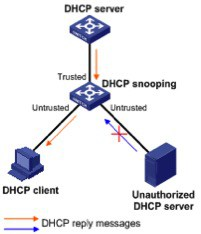
\includegraphics[width=150px]{pic/dhcpsnooping.jpg}
    \caption{DHCP Snooping.}
    \label{fig:dhcp_snooping}
\end{figure}

\section{Implementácia}
Prvým implementovaným útokom je útok \textbf{DHCP Starvation}. Ide o vyčerpanie voľných adries legitimného DHCP servera. V prvom kroku je potrebné nakonfigurovať socket s potrebnými parametrami. Je nutné nastaviť znovupoužívanie portu, povoliť odosielanie broadcastu a nabindovať socket na zadané rozhranie pomocou vstupného argumentu programu. Ak sa podarí vytvoriť a nastaviť socket zostáva nainicializovať jednotlivé štruktúry pre DHCP packety. Na simulovanie DHCP komunikácie sa využíva nekonečný while cyklus, kde na začiatku sa musí vygenerovať jedinečná MAC adresa a jednoznačné identifikačné číslo komunikácie (\texttt{xid}). Následne sa môže vytvoriť DHCP Discover packet, ktorý zahajuje DHCP komunikáciu. Je naplnený dátami podľa špecifikácie RFC 2131\footnote{https://www.ietf.org/rfc/rfc2131.txt}. Na odoslanie packetu socketom sa využíva funkcia \texttt{sendto()} z knižnice \texttt{<sys/socket.h>}. DHCP Discover packet sa odosiela na broadcast s IP adresou \texttt{255.255.255.255} a portom \texttt{67}. Na prijatie DHCP Offer packetu z legitímneho DHCP servera sa využíva \textit{blokujúce} volanie funkcie \texttt{recv()}. Po prijatí je potrebné z neho získať ip adresu DHCP servera, ktorá sa nachádza v časti \texttt{DHCP options} s id \texttt{54} a ponúkanú ip adresu, ktorá sa nachádza v časti \texttt{DHCP YIADDR}. Zo získaných dát je ďalším krokom naplnenie DHCP Request packetu, ktorý sa taktiež obdobne odošle na socket a po odoslaní sa čaká na potvrdzovací packet s názvom DHCP Ack. Po prijatí Ack packetu sa použitým štruktúram vymažú všetky data aby sa mohli použiť znovu.

Druhým implementovaným útokom je útok \textbf{DHCP Rogue}. Cieľom aplikácie je na danom rozhraní prevádzkovať DHCP server, ktorý bude žiadateľom o IP adresu poskytovať vlastnú sadu sieťových parametrov. Prvým krokom je taktiež konfigurácia socketu s potrebnými parametrami. Oproti prvému útoku sa navyše nastaví timeout na hodnotu 3600s. Počas tohto času program čaká na DHCP Discover packet. Po uplynutí tohto času funkcia \texttt{recv()} vráti chybu a program sa ukončí. V tomto kroku je potrebné zistiť priradenú IP adresu, broadcast adresu a MAC adresu zariadenia aby sme vedeli generovať korektné DHCP packety. K tomuto kroku sa využíva prístup na najnižšiu úroveň sieťových zariadení v Linuxe za pomoci knižnice \texttt{netdevice} \footnote{http://man7.org/linux/man-pages/man7/netdevice.7.html}. Po konfigurácií socketu, získaní všetkých relevantných dát sa môže inicializovať DHCP komunikácia. Princíp je veľmi podobný nekonečnému while cyklu v prvom programe. Výnimkou je, že komunikáciu v tomto prípade inicializuje klient. Program čaká v \textit{blokujúcom} volaní funkcie \texttt{recv()} na DHCP Discover packet. Po úspešnej komunikácií sa inkrementuje ponúkaná IP adresa, ktorá bola získaná zo vstupných parametrov. Program skončí ak sa minul celý rozsah ponúkaných adries.

\section{Demonštrácia činnosti}

Celková implementácia a demonštrácia činnosti prebiehala vo virtualizačnom prostredí VirtualBox s využitím virtuálnej mašinky \texttt{ISA2015.ova}. Na predvedenie funkčnosti programov som si nasimuloval sieť zobrazenú na obrázku \ref{fig:diagramsite}. Na odchytenie DHCP packetov som využil program Wireshark\footnote{https://www.wireshark.org}.

\begin{figure}[h]
    \centering
    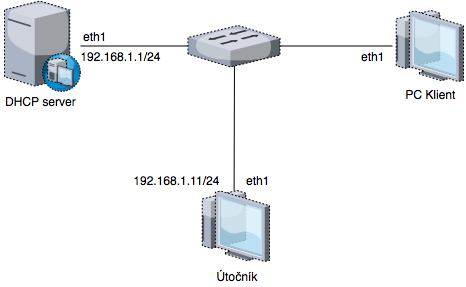
\includegraphics[width=300px]{pic/diagramsite.png}
    \caption{Topológia siete.}
    \label{fig:diagramsite}
\end{figure}

Pre úspešný útok a odstavenie DHCP serveru je potrebné spustiť najprv DHCP Starvation útok a potom DHCP Rogue útok. Po nenápadnom pripojení do siete a obdržaní IP adresy od legitímneho servera môžeme začať s prvým útokom. V simulovanej topológií sa zatial nenachádza žiadny klient. Program spustíme pomocou príkazu \texttt{sudo ./pds-dhcpstarve -i eth1}. Po vyčerpaní adresného poolu legitímneho DHCP serveru môžeme program korektne ukončiť pomocou signálu \texttt{SIGINT}~(Obr.~\ref{fig:0}).

\newpage
\begin{figure}[h]
    \centering
    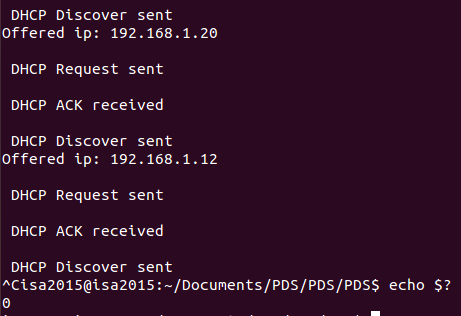
\includegraphics[width=300px]{pic/0.png}
    \caption{Ukončenie programu.}
    \label{fig:0}
\end{figure}

Pri odchytení komunikácie v programe Wireshark môžeme vidieť ako komunikácia prebiehala (Obr.~\ref{fig:1}. Program generoval DHCP Discover packety až pokiaľ nevyčerpal adresný pool DHCP servera.

\begin{figure}[h]
    \centering
    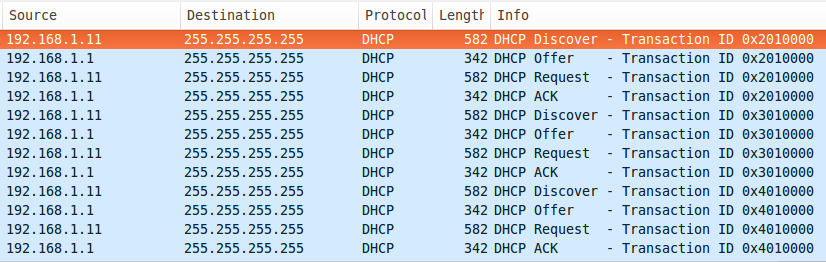
\includegraphics[width=400px]{pic/1.png}
    \caption{DHCP komunikácia pri starvation útoku.}
    \label{fig:1}
\end{figure}

\newpage

Nový pripojený klient do siete očakáva IP adresu od DHCP servera. Ako je možné vidieť na obrázkoch \ref{fig:2} a \ref{fig:3} žiadnu adresu neobdrží - legitimný DHCP server má vyčerpaný adresný pool poskytovaných adries.

\begin{figure}[h]
    \centering
    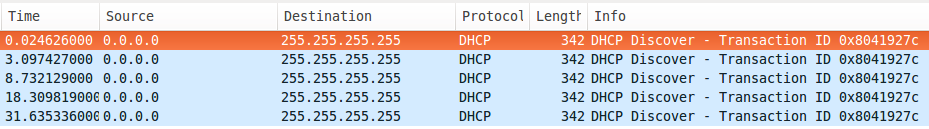
\includegraphics[width=400px]{pic/2.png}
    \caption{Klient posiela DHCP Discover packety.}
    \label{fig:2}
\end{figure}

\begin{figure}[h]
    \centering
    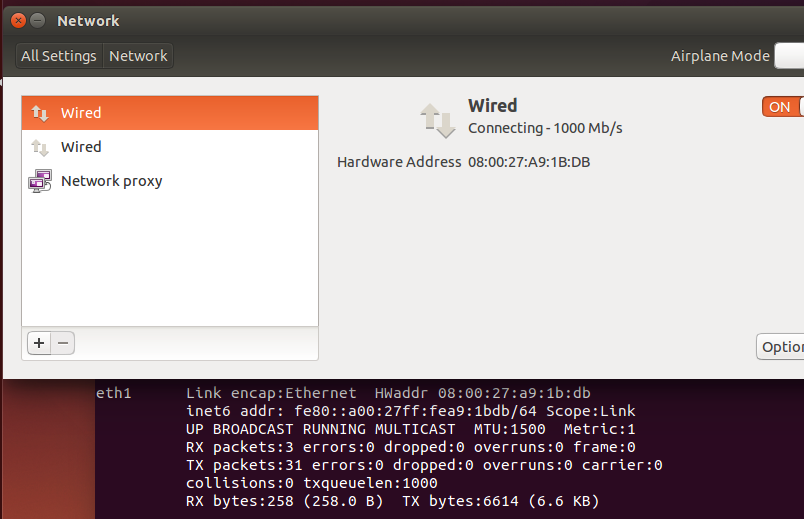
\includegraphics[width=400px]{pic/3.png}
    \caption{Klient je bez IP adresy.}
    \label{fig:3}
\end{figure}

 Momentálne je legitímny DHCP server úplne odstavený. Na radu môže prísť DHCP rogue útok. Program spustíme pomocou príkazu \texttt{sudo ./pds-dhcprogue -i eth1 -p 192.8.100.100-192.168.100.200 -g 192.168.1.1 -n 8.8.8.8 -d fit.vutbr.cz -l 3600}. Od tohto momentu každý novo pripojený klient získava podvrhnuté informácie (Obr.~\ref{fig:4}, Obr.~\ref{fig:5}).

\begin{figure}[h]
    \centering
    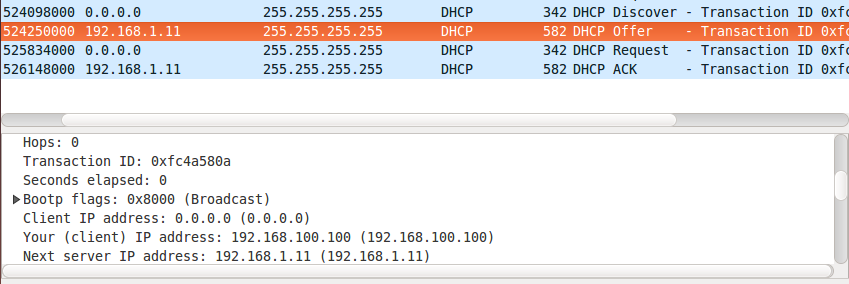
\includegraphics[width=400px]{pic/8.png}
    \caption{Klient dostal podvrhnutú IP adresu.}
    \label{fig:4}
\end{figure}

\begin{figure}[h]
    \centering
    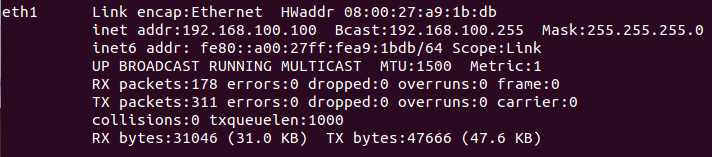
\includegraphics[width=400px]{pic/9.png}
    \caption{Klientovo rozhranie.}
    \label{fig:5}
\end{figure}

Finálna schéma topológie po korektnom vykonaní obi dvoch útokov je zobrazená na obrázku \ref{fig:diagramsite2}.

\begin{figure}[h]
    \centering
    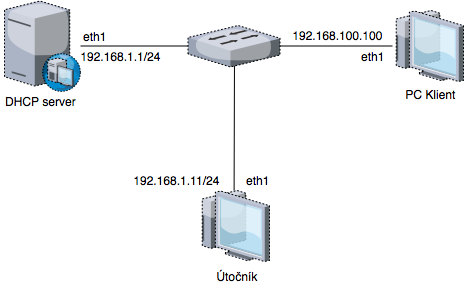
\includegraphics[width=300px]{pic/diagramsite2.png}
    \caption{Topológia siete po útoku.}
    \label{fig:diagramsite2}
\end{figure}

\newpage
\bibliography{literatura}
\end{document}
